

\documentclass[11pt,twocolumn]{article} 
\usepackage{fancyhdr}
\usepackage{expl3,xparse,xcoffins,titling,kantlipsum}
\ExplSyntaxOn
\coffin_new:N \l_my_abstract_coffin
\dim_zero_new:N \l_my_width_dim
\keys_define:nn { my / abstract }
  {
    width .code:n = {
      \dim_set:Nn \l_my_width_dim {#1\textwidth}
    }
  }
\NewDocumentCommand \myabstract { O {width=.8} m }{%
  \keys_set:nn { my / abstract } { #1 }
  \SetVerticalCoffin \l_my_abstract_coffin {\l_my_width_dim} {#2}
  \renewcommand\maketitlehookd{%
    \mbox{}\medskip\par
    \centering
    \TypesetCoffin \l_my_abstract_coffin
  }
}
\ExplSyntaxOff
\usepackage[document]{ragged2e}
\usepackage{geometry}
 \geometry{
  a4paper,
  total={170mm,257mm},
  left=17.5mm,
  right=17.5mm,
  bottom=15mm,
  top=15mm
 }
 
% \documentclass{gji}
\usepackage{amssymb}
\usepackage{enumitem}
\usepackage{amsthm}
\usepackage{amsmath}
\usepackage{timet,color}
\usepackage{nomencl}
\setlength{\nomitemsep}{-\parsep}
\usepackage{graphicx}
\usepackage[urlcolor=blue,citecolor=black,linkcolor=black]{hyperref}
\usepackage[english]{babel}
\usepackage{times}
\usepackage{multicol}
\makenomenclature
\begin{document}

\title{\bf \Huge Exploring Logistic Map and Chaos.}
\author{{\bf \Large Nicholas Cotton}\\
  MATH 497
  }
\date{April 17th 2024}


\let\leqslant=\leq

\label{firstpage}


%%
%% This format for begin abstract is a reclaration of a macro to 
%% create single columne for abstract
%%
%\myabstract[width=.7]{
%This report presents a comprehensive exploration of the logistic map within the context of dynamical systems. The logistic map is often used in understanding population dynamics and other complex phenomena. Through detailed analysis, the report covers key topics including stability analysis, bifurcation phenomena, chaos theory, sensitive dependence on initial conditions, attractors, and real-world applications. Overall, this report aims to provide solid grasp of the logistic map and why it's important in the world of dynamical systems.
%\noindent
%{\bf Keywords:} Authors are advised to write 3-5 keywords related to the project, separated by comma. 
%}


\maketitle

%%
%% This creates a header title for MECH0020_AY2023-24
%%
\pagestyle{fancy}
\fancyhead[L]{MATH497\underline{\hspace{.1in}}SPR2024}
\fancyhead[R]{COTTON}
%%
%% This creates the nomenclature list - dont forget to tag the 
%% definitions for new symbols as you go through
%%

%\printnomenclature

\section{Introduction}

The logistic map is a classic example of a dynamical system used to study populations. Popularized in a 1976 paper by biologist Robert May\cite{May1976}
, the logistic map is a dynamical system described by the function $f:[0,1]\to[0,1]$ defined as
\[f(x)=rx(1-x)\]
or more commonly written,
\begin{equation}
x_{n+1} = rx_n(1-x_n) \label{eqn:equation1}
\end{equation}
where
\begin{itemize}
    \item $x_n$ is the (normalized) population at time n. 
    \item $r$ is a parameter that controls the rate of population growth. We focus on $0\leq r\leq 4$
    \item Both a growth term $rx_n$ and a limiting factor $(1-x_n)$
\end{itemize}
\subsection{Just a parabola?}
You might notice that the logistic map is actually just a parabola.
Reformulating the equation as $f(x)=rx(1-x)=rx-rx^2$ we can clearly see that logistic map is simply a quadratic. This parabola achieves a maximum value at $x_{max}=\frac{1}{2}$. Plugging in $x_{max}$, we can easily solve for this maximum value in terms of $r$.
\begin{equation}
    f(x_{max})=\frac{r}{2}(1-\frac{1}{2})=\frac{r}{4}
\end{equation}

This behavior can be seen in Figure 1 and also explains why we consider $0\leq r\leq 4$.



\begin{figure}
    \centering
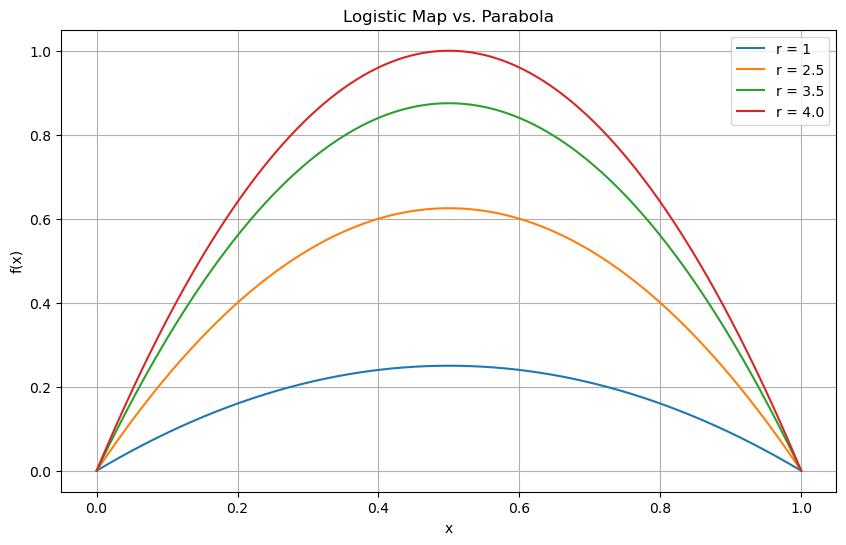
\includegraphics[width=0.45\textwidth]{figures/parabolas.png}
    \caption{Plot of Logistic Map for various $r$}
    \label{fig:enter-label}
\end{figure}


\section{Stability and Bifurcation Analysis}
\subsection{Stability}
In stability analysis, we want to study the long term behavior of a dynamical system and how it responds to small perturbations in our initial values.
In the context of the logistic map, we examine the stability of its fixed and periodic points.
To do this, we consider the first order Taylor series expansion around a fixed point $x^\ast$
\begin{equation}
    x_{n+1}=f'(x^\ast)(x_n-x^\ast)+x^\ast
\end{equation}
where $f'(x^\ast)$ is the derivative of the logistic map at $x^\ast$.

We can see that if $|f'(x^\ast)|<1$ , the fixed points are stable since points around them will converge to the fixed point.


Here, we explore the stability of periodic points across distinct ranges of the parameter $r$.


\subsubsection{$r < 1$}
When $r<1$, there is an obvious fixed point at $x^\ast=0$.
Taking the derivative, we can see that $x^\ast$ is stable.
\begin{equation}
f'(x)=\frac{d}{dx}rx_n(1-x_n)=\frac{d}{dx}r(x-x^2)=r(1-2x)
\end{equation}

Note that for any $x\in[0,1]$, $|f'(x)|<1$, and so $f$ is a contraction on $[0,1]$
\[|f(x)-f(y)|\leq r|x-y|\]

Figure 2 shows this behavior for $r=0.5$ and various initial conditions.

Note that for $r=1$, orbits also converge to 0.

\begin{figure}
    \centering
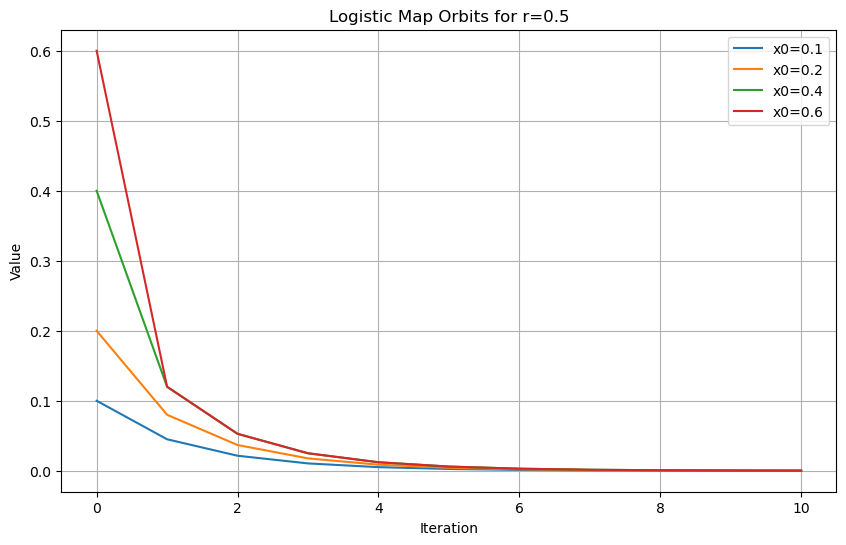
\includegraphics[width=0.45\textwidth]{figures/rles1.png}
    \caption{Orbits for $r=0.5$}
    \label{fig:enter-label}
\end{figure}

\subsubsection{$1 < r < 2$}
When $1 < r < 2$, we still have our obvious fixed point at 0, however, when we check the stability at $x=0$,
\[|f'(0)|=r\geq 1\]
Thus $0$ is not a stable fixed point.

Lets see if we cannot find other fixed points.
Solving $x^\ast=rx^\ast(1-x^\ast)$ for $x^\ast$ gives us
\begin{equation}
x^\ast=\frac{r-1}{r}
\end{equation}
We have found our fixed point!
Checking stability at $x^\ast$ using $(4)$ gives,
\[f'(x^\ast)=r(1-2x^\ast)=r(1-2\frac{r-1}{r})=\frac{2-r}{r}\]
We can see that when $1 < r< 2$,
\[|f'(x^\ast)|< 1\]
So $x^\ast=\frac{r-1}{r}$ is a stable fixed point and all orbits will converge to $x^\ast$

We can see this behavior when $r=1.5$ in Figure 3 

\begin{figure}
    \centering
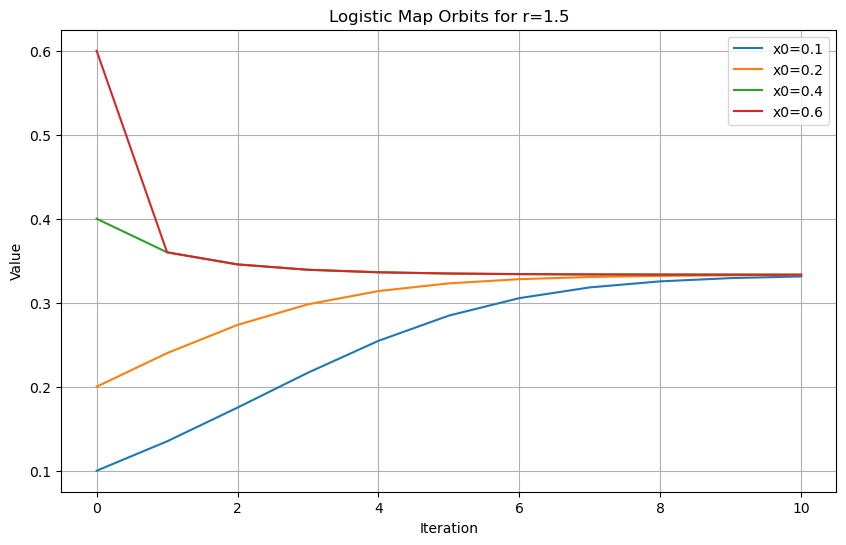
\includegraphics[width=0.45\textwidth]{figures/1lesrles2.png}
    \caption{Orbits for $r=1.5$}
    \label{fig:enter-label}
\end{figure}

\subsubsection{$2\leq r<3$}
Performing the same analysis for $2\leq r < 3$ gives us the same results however we see some oscillations in the orbits before they finally converge to $x^\ast=\frac{r-1}{r}$.
While no points are periodic (except the fixed point itself), these oscillations hint at possible periodicity in other ranges for $r$.

We can see this behavior for $r=2.8$ in Figure 4

\begin{figure}
    \centering
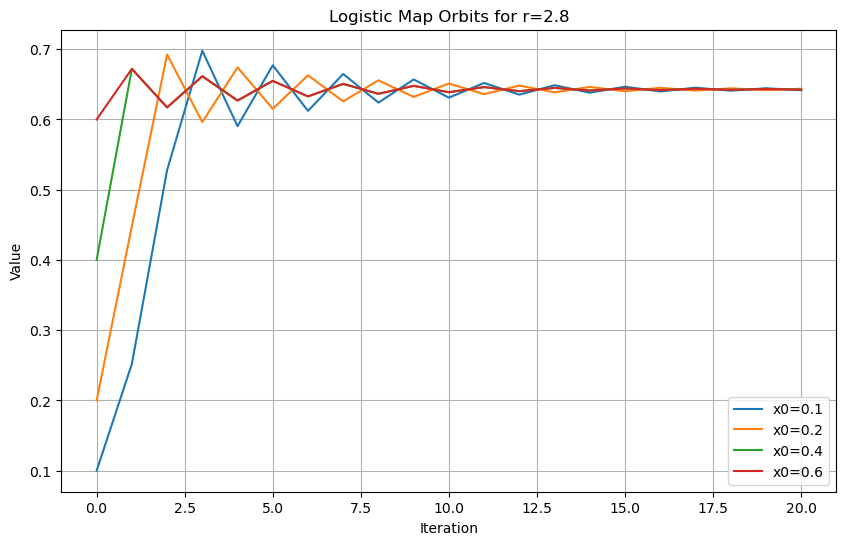
\includegraphics[width=0.45\textwidth]{figures/2lesrles3.png}
    \caption{Orbits for $r=2.8$}
    \label{fig:enter-label}
\end{figure}
\subsubsection{$3\leq r<4$}
This is where things get intersting.

In the $3\leq r<4$ case we see many different intersting behaviors occur

Firstly, for $3\leq r\leq 1+\sqrt{6}$, we find two stable periodic points of period two at,
\begin{equation}
	x_\pm = \frac{1}{2r}(r+1\pm \sqrt{(r-3)(r+1)})
\end{equation}
\cite{TsuchiyaYamagishi}

After that, we find a region with four stable periodic points of period $4$, and after that we find a region with eight stable periodic points of period $8$.
This doubling of period points continues until $r\approx 3.56995$. Well call $3.56995...= a$ 
This region of $3\leq r<a$ is commonly refered to as the "period doubling cascade."

$r>a$ is known as the chaotic region of the logistic map, we find that almost every orbit is dense with unstable periodic points.

All of these behaviors can be seen in the bifurcation diagram (Figure 5)
\begin{figure}
    \centering
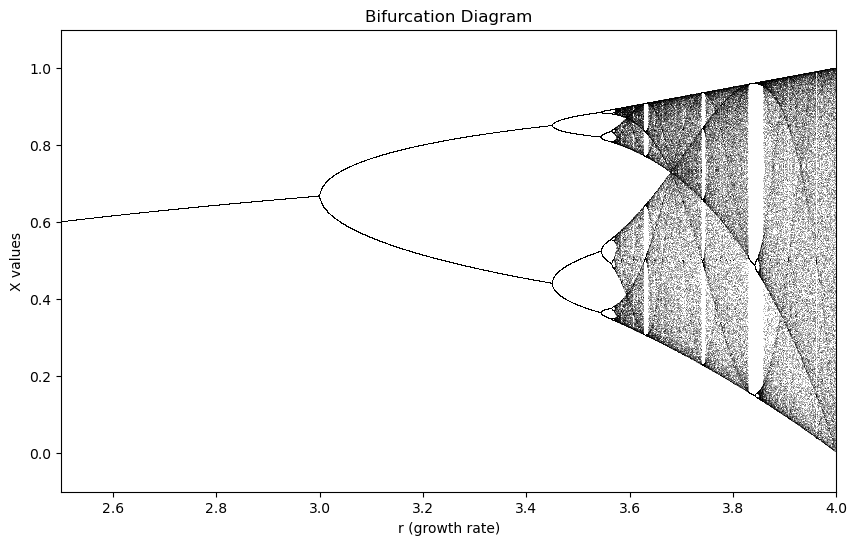
\includegraphics[width=0.45\textwidth]{figures/bifurcations.png}
    \caption{Bifurcation diagram for $r$}
    \label{fig:enter-label}
\end{figure}
\subsection{Bifurcations}
So why does this happen? How can this seemingly simple parabola have such interesting dynamics?

One way to better understand the dynamics, is to study the bifurcations that occur as we adjust $r$. In the previous section we listed various regions of $r$ that result in different long term behavior for the logistic map.
This is precisely what we want to study in more depth with Bifurcation analysis.
Bifurcation analysis explores the qualitative changes in the behavior of a dynamical system as a parameter, such as $r$ in the logistic map, is varied. We hope to identify critical values of the parameter where transitions occur, leading to the emergence of different behaviors.
\subsubsection{Bifurcation Diagram}
Figure 5 provides an interesting numerical result that helps us to visualise the changes in behavior of the logistic map for different values of $r$.
This diagram is generated by fixing $x_0$ and iterating through the logistic map $1000$ times, (this way we can ensure we are looking at the long term behavior of the system) then plotting the next $100$ iterates of the map; we do this for each value of $r$.

Note that Figure 5 only includes values of $r$ starting from $2.5$ since we have already discussed the bifurcation from our single stable fixed point at $0$ for $r<1$, to our single stable fixed point at $\frac{r-1}{r}$.
\subsubsection{Period Doubling Bifurcations and Feigenbaum constant.}
As $r$ increases past the critical value of $3$, the process of period doubling repeats itself iteratively. Each successive bifurcation creates a new stable orbit with double the period of the previous orbit. This results in a "cascade of period doubling", where the system transitions from period-1 to period-2, period-2 to period-4, period-4 to period-8, and so on.

One interesting property of this period doubling is its universal scaling.
As the system approaches chaos, the widths of period $n$ regions get smaller and smaller until they converge to 0; however, the ratios of the width of each region to the width of the previous region converges to a constant $\delta\approx 4.6692$.
$\delta$ is known as Feigenbaum constant.
This can be found by taking 
\begin{equation}
\lim_{k\to\infty}\frac{r_{k-1}-r_{k-2}}{r_k-r_{k-1}}
\end{equation}
where $r_k$ are discrete values of $r$ at the $k^{th}$ period doubling.
Interestingly, we also see similar period doubling and the \emph{same} $\delta$ for all systems of similar form (parameter times some (quadratic-like) nonlinear term.). 
\cite[p.~503]{AlligoodSauerYorke}.

Period doubling bifurcations serve as a precursor to chaotic behavior in the logistic map. As $r$ increases beyond the accumulation point of period doubling, the system enters a region of chaotic dynamics characterized by sensitivity to initial conditions and a lack of long-term predictability.




\begin{figure}
    \centering
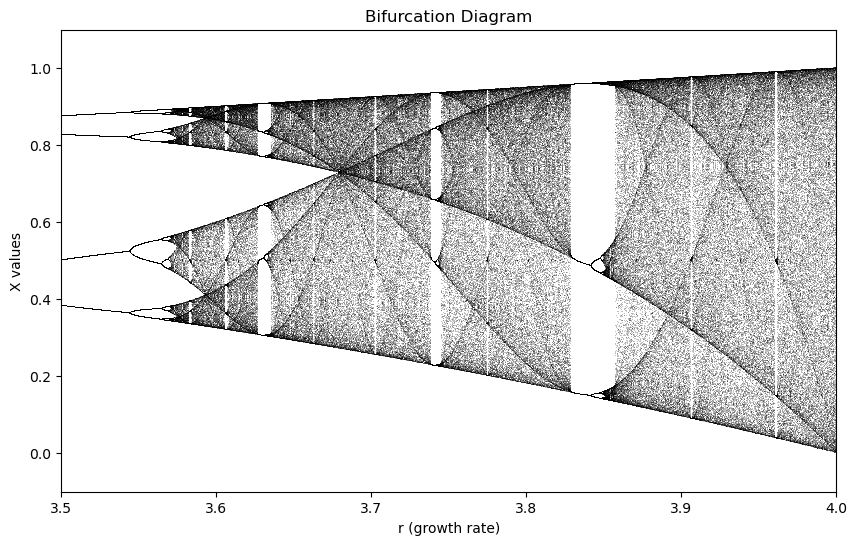
\includegraphics[width=0.45\textwidth]{figures/chaosregion.png}
    \caption{Chaotic region of Logistic Map}
    \label{fig:enter-label}
\end{figure}
\begin{figure}
    \centering
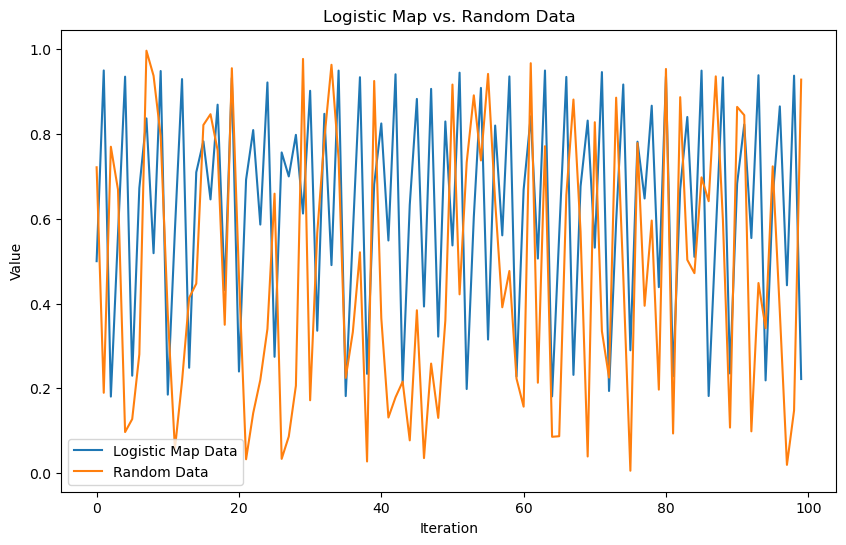
\includegraphics[width=0.45\textwidth]{figures/logvsrand.png}
    \caption{Logistic Map vs. Random Data (1)}
    \label{fig:enter-label}
\end{figure}



\section{Chaos}
Remember we called $a=3.56995...$.
In this section we focus on the chaotic region of $r>a$.
Figure 6 shows the bifurcation diagram in this region.

In chaos theory, a system is said to be chaotic if it displays sensitive dependence on initial conditions, topological mixing, and dense orbits.
The Logistic Map is said to have deterministic chaos since there is no \emph{randomness} involved. Rather the orbit of a point is entirely determined by initial values and conditions.
\cite[p.~252]{AlligoodSauerYorke}
\subsection{Randomness vs. Chaos}
Figure 7 plots the orbit of the logistic map with $r=3.8$ and $x_0=0.5$ against random data generated by $np.random.rand()$.
When looking at the orbits its hard to differentiate the two curves; both seem to have random behavior. 

However, when we plot $x_n$ against $x_{n+1}$, as in Figure 8, the logistic map shows a behavior that is determined entirely by the equation itslef, while the random data just looks like noise.
This type of plot of $x_n$ against the next iteration is commonly refered to as a Poincare Plot.

\subsection{Topological Mixing and Dense Orbits for the case of $r=4$}
A map $f:X\to X$ is topologically mixing if for any non-empty open sets $U,V\subseteq X$,
\[f^n(U)\cap V\neq \emptyset\]
for sufficiently large n.

A point has orbit dense in $X$ if it visits every open interval in $X$.


To prove these properties for the case of $r=4$ we first consider that the map is topologically semiconjucate to $E_2(x)=2x\mod 1$
\begin{figure}
    \centering
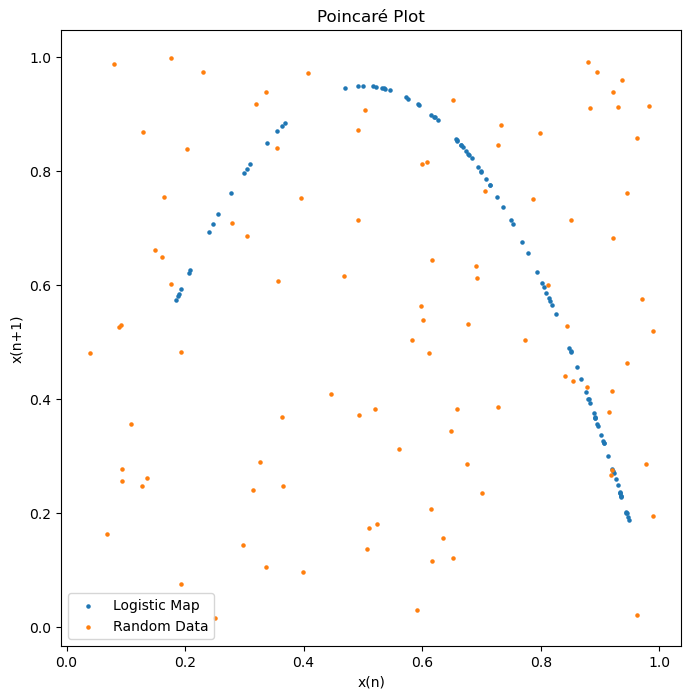
\includegraphics[width=0.45\textwidth]{figures/Poincare.png}
    \caption{Logistic Map vs. Random Data (2)}
    \label{fig:enter-label}
\end{figure}
\begin{figure}
    \centering
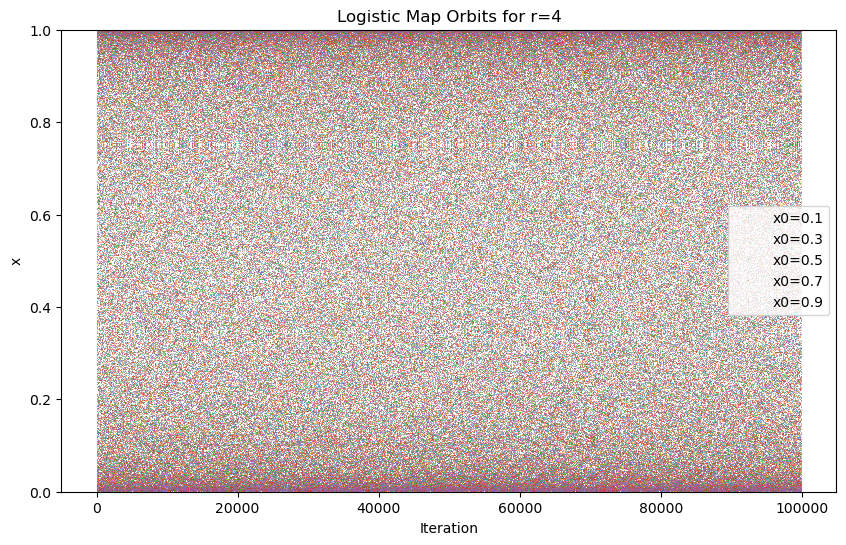
\includegraphics[width=0.45\textwidth]{figures/denseorbits.png.png}
    \caption{Dense orbits of $r=4$}
    \label{fig:enter-label}
\end{figure}

\begin{proof}
	\item {Presented my findings.}
	Here we will define $f:[0,1]\to[0,1]$ as in $(8)$ with $r=4$.
	We want to show that $f$ is topologically semi-conjugate to $E_2(x)=2xmod 1$ on $S^1$. From there we can take orbits of the logistic map to orbits of $E_2$ and show that $E_2$ is topologically mixing.

	To show that $f$ and $E_2$ are topological semiconjugates we need to show that there is $h$ s.t.
	\[h\circ E_2=f\circ h\]
	Consider $h=\sin^2\pi x$ and
	\begin{equation}
	h(2x)=f(\sin^2\pi x)\text{ for }0\leq x\leq \frac{1}{2}
	\end{equation}
	\begin{equation}
	h(2x-1)=f(\sin^2\pi x)\text{ for }\frac{1}{2}\leq x\leq 1
	\end{equation}
	Cosider the right hand side of both equations.
	\[f(\sin^2\pi x)=4(\sin^2\pi x)(1-\sin^2\pi x)=\]
	\[=4(\sin^2\pi x)(\cos^2\pi x)=\]
	\[=4(\frac{1}{2}-\frac{1}{2}\cos2\pi x)(\frac{1}{2}+\frac{1}{2}\cos2\pi x)=\]
	\[=4(\frac{1}{4}-\frac{1}{4}\cos^22\pi x)=\]
	\[=4(\frac{1}{4}\sin^22\pi x)=\sin^22\pi x\]
	The left hand side for $(9)$ is $h(2x)=\sin^2\pi(2x)=\sin^22\pi x$.
	The left hand side for $(10)$ is $h(2x-1)=\sin^2\pi(2x-1)=\sin^2(2\pi x-\pi)=\sin^22\pi x$
	
	Thus $f$ and $E_2$ are topologically semiconjugate via $h=\sin^2\pi x$.
	Now, for any arc $U$ in $S^1$, $E_2^n(U)=S^1$ for sufficiently large $n$, and so $E_2$ is topologically mixing.
	Therefore, $f$ is topologically mixing.

	Furthermore, since $h$ is continuously differentiable, it follows that  for $f$, almost every point has dense orbit.



\end{proof}

Numerically, we can show that orbits are dense by simply plotting the orbit of several initial values and seeing that their orbits fill up the space.
Figure 9 shows 100000 iterations after an initial 100 iteration "burn in period" for 5 initial values when $r=4$.
\subsection{Sensitivity to initial conditions}
Sensitive dependence on initial conditions means that small perturbations in the initial value $(x_0)$ lead to significantly different long-term outcomes.

This sensitivity is expressed by exponential divergence of orbits. For any two initial values $x_0$ and $x'_0$, the distance between their orbits grows exponentially as $n$ increases.
Formally, this means that there exists some $\lambda$ such that,
\begin{equation}
	|x_n-x'_n|\approx e^{\lambda n}|x_0-x'_0|
\end{equation}

$\lambda$ is called the Lyapunov Exponent.

\cite{Czornik2013}

We can also simply look at the orbits of two nearby intial values and clearly see that the long term behaviors are completely different. (Figure 10)
\begin{figure}
    \centering
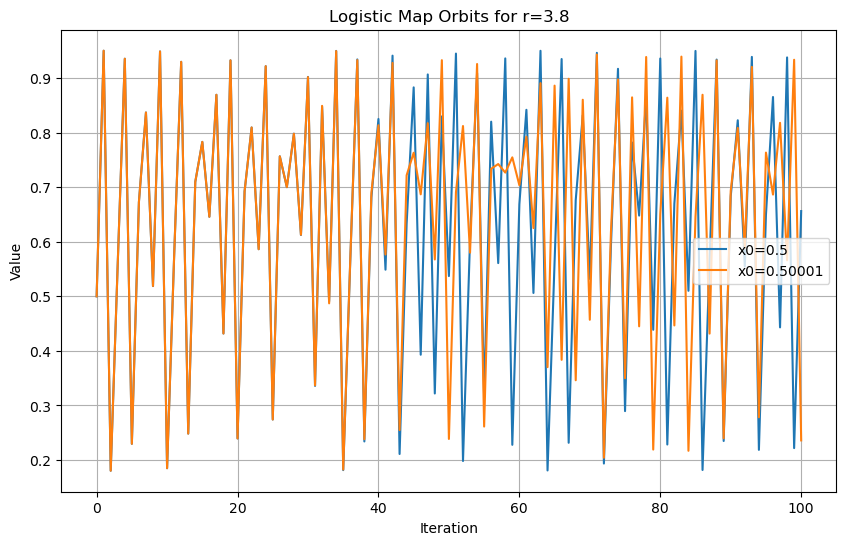
\includegraphics[width=0.45\textwidth]{figures/sensitivity.png}
    \caption{Orbits of close initial values}
    \label{fig:enter-label}
\end{figure}
\begin{figure}
    \centering
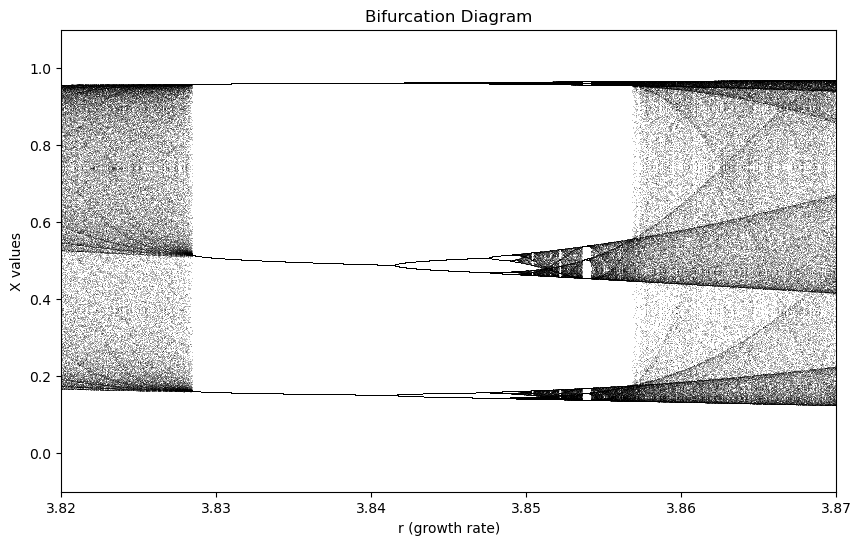
\includegraphics[width=0.45\textwidth]{figures/p3region.png}
    \caption{Stable period $3$ orbits in chaos}
    \label{fig:enter-label}
\end{figure}
\subsubsection{Lyapunov Exponent}
The Lyapunov exponent measures how quickly initially nearby points diverge from each other as the system evolves over time.
A positive Lyapunov exponent indicates exponential divergence, meaning that nearby orbits will separate exponentially with time.
Conversely, a negative Lyapunov exponent indicates convergence, where nearby orbits approach each other exponentially. 

For the logistic map, positive Lyapunov exponents in the chaotic region indicate sensitive dependence on initial conditions and exponential divergence of orbits.
This is consistant with its chaotic behavior.

We can easily compute Lyapunov exponent using
\begin{equation}
	\lambda = \lim_{n\to\infty}\frac{1}{n}\sum^n_{i=1}\ln|f'(x_i)|
\end{equation}

\cite{Czornik2013}

\subsection{Stable Period-3 Orbit Emerges}
Remarkably, suddenly at $r=1+\sqrt{8}\approx3.8284$, a stable period-3 periodic point emerges.
\cite{Bechhoefer}
We can even check the Lyapunov exponents in this region and see that they are negative, showing us that orbits will converge.
Zooming into this area of the bifurcation diagram (Figure 11) shows that we do infact have a stable period 3 orbit emerge. We also see the same period doubling that we saw in the $3\leq r<a$ region before quickly returning to chaos.

\section{Attractors and Fractals}
\subsection{Attractors}
In the bifurcation diagram, we can see that the orbits, while not converging to a single point, converge to some bounded region. This region is called an attractor.

Formally, for a function f:X\to X$, an attractor is a subset $A$ of $X$ such that

"
\begin{enumerate}[label=(\roman*)]
	\item
		If $a\in A$, then $f^n(a)\in A$ for all $n\in\mathbb{N}$ 
	\item
		There exists a neighborhood of $A$, called the \emph{basin of attraction} for $A$ and denoted $B(A)$, which is the set of all points $b\in X$ with the following property: for any open set $U$ containing, $A$, there exists $N\in\mathbb{N}$ s.t. $f^n(b)\in U$ for all $n\geq N$
	\item
		There is no proper (non-empty) subset of $A$ having the first two properties.
	
\end{enumerate}
"

\cite{wikiAttractor}
\subsubsection{Fractal Dimension}
One way to quantitatively measure the \emph{strangeness} of the attractor is with \emph{Fractal Dimension}.
Fractal dimensions are a way of characterizing the complexity or fractal nature of a geometric object.
"Generally speaking, we may think of the dimension as giving in some way, the amount of information necessary to specify the position of the point on the attractor to within a given accuracy."
\cite{Sarmah2014}

The method we will use is called the box counting dimension.

The \emph{box-counting dimension} of a bounded set $X$ in $\mathbb{R}$ is
\[dim_B(X)=\lim_{\epsilon\to0^+}\frac{\ln N(\epsilon)}{\ln(1/\epsilon)}, \text{ if the limits exists,}\]
where $N(\epsilon)$ is the least number of boxes with side $\epsilon$ needed to cover $X$.
If the limit does not exist, we consider the upper and lower box dimensions defined as the cooresponding $\liminf$ and $\limsup$.
\cite{Falconer2013}
Solving for this numerically gives a result of around $0.559$ when $r=3.5699456$.
We can find comfort in this result as more a precise dimension, called Hausdorff dimension, has a known value of around $0.538$ for logistic map at $r=3.5699456$\cite{Grassberger1981}


\subsection{Self Similarity}
The bifurcation diagram is self similar. If we zoom in on any non-chaotic point we will see that it looks like the full diagram.
In [10]\cite{youtube}, the bifurcation diagram of the logistic map is zoomed in by a factor of 1 million, showcasing its self similarity.



\section{Conclusion}
In conclusion, the logistic map, a model for population dynamics, displays a variety of behaviors determined by a single parameter, $r$. Through stability and bifurcation analysis, we see how small changes in $r$ lead to significant shifts in the system's behavior, from stable points to periodic orbits and eventually to chaotic dynamics.

The chaotic region, characterized by sensitivity to initial conditions, demonstrates the map's deterministic yet unpredictable nature. Despite this unpredictability, stable periodic orbits can emerge intermittently amidst the chaos.

Furthermore, the logistic map reveals self-similar structures known as strange attractors and fractals, showcasing the underlying order within apparent randomness.





\bibliographystyle{IEEEtran}

% \bibliographystyle{ieeetr}
\bibliography{manuscript_references}

\end{document}
